\section{Trigger} 
\label{sec:trigger}

The data used in this analysis is collected using triggers that are designed to collect events with high $\ptmiss$ and $\htmiss$. 
These triggers rely on the online version of the Particle Flow algorithm. While calculating $\ptmiss$ and $\htmiss$, identified
Particle Flow muons are removed from the event. Therefore, using the same triggers, one can also select dimuon (Z \rightarrow \mu \mu) 
and single muon (W \rightarrow \mu \nu) events.

The remaining control regions include dielectron (Z \rightarrow ee) and single electron (W \rightarrow e\nu) regions. In these two control
regions, events are selected using the Single Electron trigger. The full list of triggers used in this analysis are given in 
Tab.~\ref{tab:triggers}.

\begin{table}[ht!]
    \centering
    \small
    \def\arraystretch{1.5}
    \caption{HLT paths, and the associated L1 seeds being used in the analysis.}
    \begin{tabular}{l l c}
        \hline
        \hline
                                &                                               \\
        HLT Path                & L1 Seed                   & Primary Dataset   \\
        % Complete the table
        
    \end{tabular}
    
\end{table}

\subsection{Overview of $\met$ triggers}

The $\ptmiss$ and $\htmiss$ based triggers are designed to maximize the signal acceptance. These triggers are seeded at L1 level using
a logical OR of available ETM based seeds. % Add more info about the L1 seeds here

% More info to be added here

\subsection{Efficiency turn-on curves}

The performance of $\ptmiss + \htmiss$ based triggers is measured by using both single muon and double muon events, i.e. sample enriched in
$W \rightarrow \mu\nu$ and $Z \rightarrow \mu\mu$ decays, respectively. The measurement is performed by using both data and MC samples 
for 2017 and 2018, seperately.

$W \rightarrow \mu\nu$ events are selected from Single Muon dataset and WJetsToLNu MC sample. % might add more info about MC sample
The muon must must pass the tight ID requirement. In addition, the transverse mass of the muon must not exceed $160 \ GeV$. 
$Z \rightarrow \mu\mu$ events are selected from Single Muon dataset and ZJetsToLL MC sample. % might add more info about MC sample
For this category of events, there must be at least one muon that is passing the tight ID requirement, and there must be exactly 
2 loose muons. In addition to these requirements, these two muons are required to have opposite charge and have an invariant mass 
consistent with the $Z$ boson, $60 < m_{\mu\mu} < 120 \ GeV$.

In both single muon and double muon events, additional requirements are also imposed. There should be no additional leptons or photons and
b-jets identified in the event. In addition, there must be at least two jets in the event, and the leading two jets must have $\pt$ higher
than $80 \ GeV$ and $40 \ GeV$, respectively. Finally, the two leading jets must satisty $\detajj > 1.0$ and $\dphijj < 1.5$.

To understand the dependence of the turn-on curves on the two leading jets, we measured the efficiency in three different categories:

\begin{itemize}
    \item Two central VBF jets: Leading two jets both satisfying $|\eta| \leq 2.4$
    \item Two forward VBF jets: Leading two jets both satisfying $|\eta| > 2.4$
    \item One central and one forward VBF jet: One of the leading jets is central with $|\eta| \leq 2.4$ and the other jet in the pair is forward 
    with $|\eta| > 2.4$
\end{itemize}

In these three categories, efficiencies are measured as a function of $\mjj$ and recoil, using both data and MC samples for 2017 and 2018,
seperately. Figs.~\ref{fig:eff_mjj_2017_1m}, \ref{fig:eff_mjj_2018_1m}, \ref{fig:eff_recoil_2017_1m} and \ref{fig:eff_recoil_2018_1m} show 
the results obtained from single muon events, whereas Figs.~\ref{fig:eff_mjj_2017_2m}, \ref{fig:eff_mjj_2018_2m}, 
\ref{fig:eff_recoil_2017_2m} and \ref{fig:eff_recoil_2018_2m} show the results obtained from double moun events.

Fig.~\ref{fig:eff_mjj_2017_1m} shows the efficiencies as a function of $\mjj$ in data and MC for the three categories in 2017, 
whereas Fig.~\ref{fig:eff_mjj_2018_1m} shows the efficiencies as a function of $\mjj$ in data and MC for the three categories in 2018. 
Fig.~\ref{fig:eff_recoil_2017_1m} shows the efficiency turn-on curves as a function of recoil in data and MC for the three categories, 
for 2017 samples, whereas Fig.~\ref{fig:eff_recoil_2018_1m} shows the efficiency turn-on curves as a function of recoil in data and MC 
for the three categories, for 2018 samples. 

\begin{figure}[htp]
    \begin{center}
        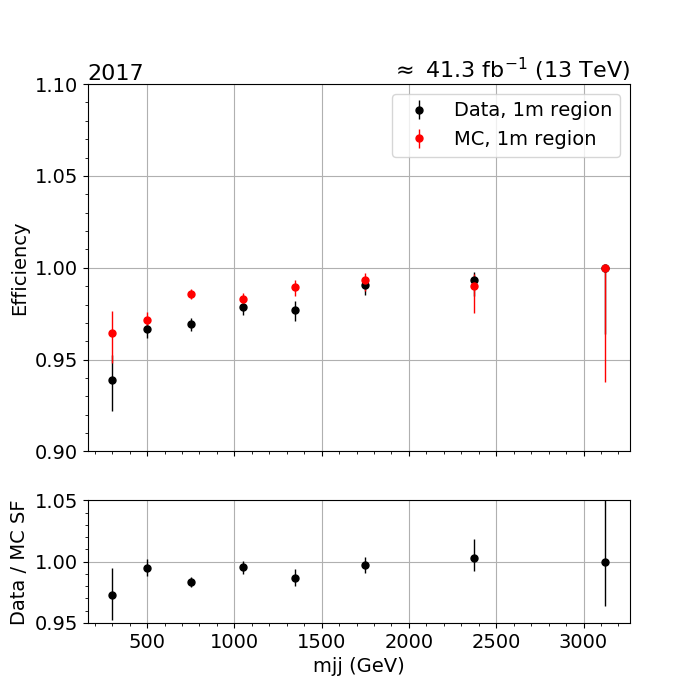
\includegraphics[width=0.49\textwidth]{fig/efficiency/trigger/met/mjj/data_mc_comparison_1m_2017_one_jet_forward_one_jet_central.png}
        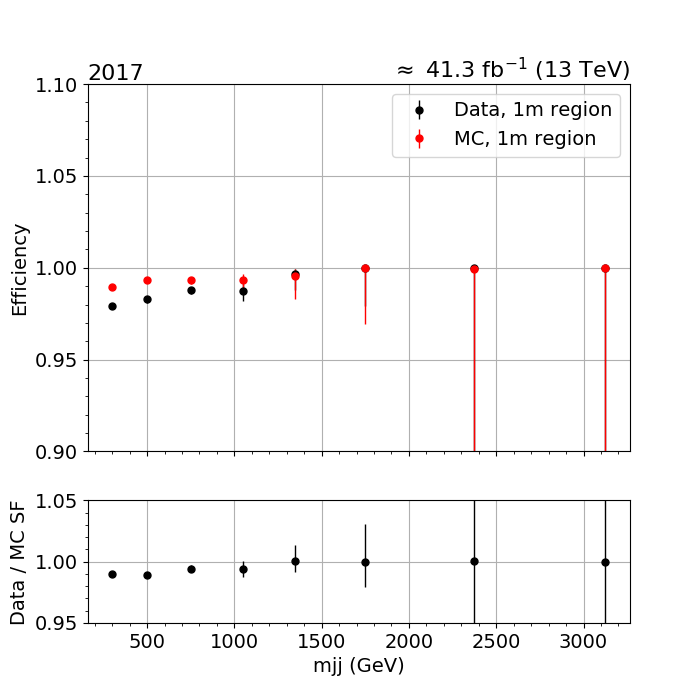
\includegraphics[width=0.49\textwidth]{fig/efficiency/trigger/met/mjj/data_mc_comparison_1m_2017_two_central_jets.png} \\
        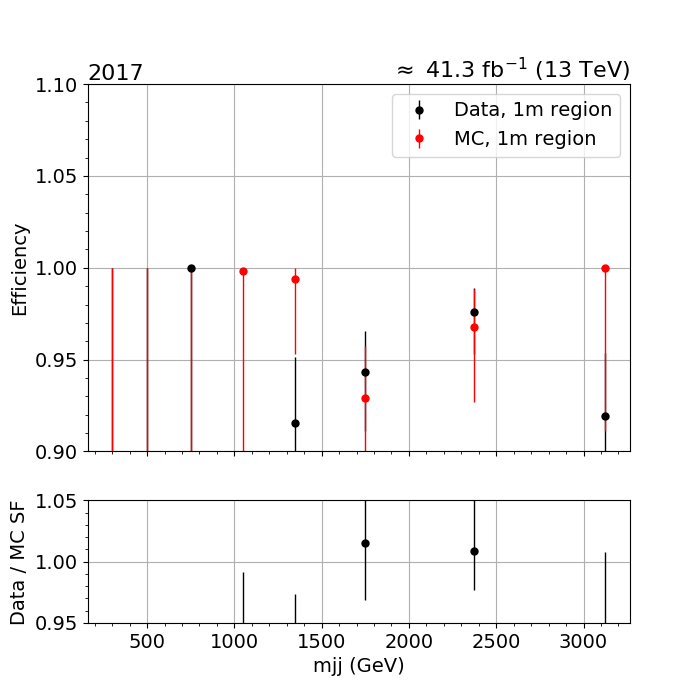
\includegraphics[width=0.49\textwidth]{fig/efficiency/trigger/met/mjj/data_mc_comparison_1m_2017_two_forward_jets.png}
    \end{center}
    \caption{MET trigger efficiency as a function of mjj in three categories: One forward jet and one central jet, two central jets and
            two forward jets. These results are obtained from 2017 data and MC samples with the selection of single muon events.} 
    \label{fig:eff_mjj_2017_1m}      
\end{figure}

\begin{figure}[hbp]
    \begin{center}
        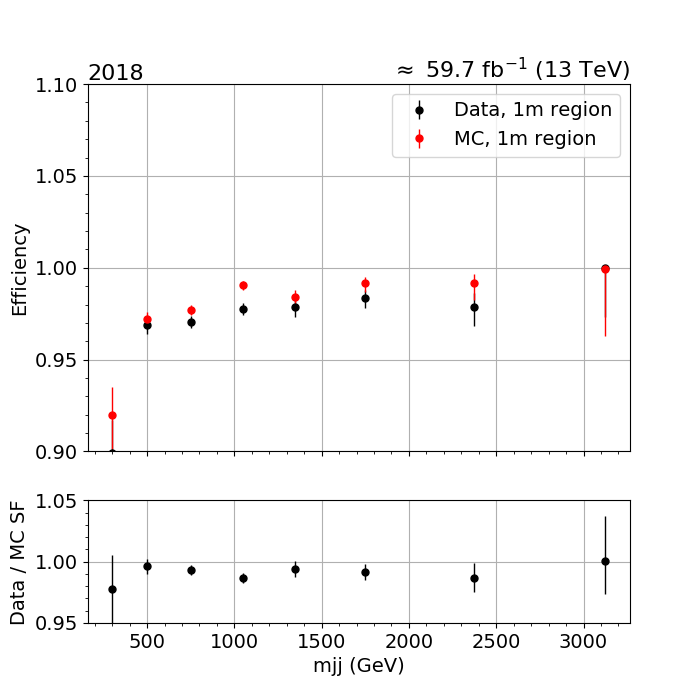
\includegraphics[width=0.49\textwidth]{fig/efficiency/trigger/met/mjj/data_mc_comparison_1m_2018_one_jet_forward_one_jet_central.png}
        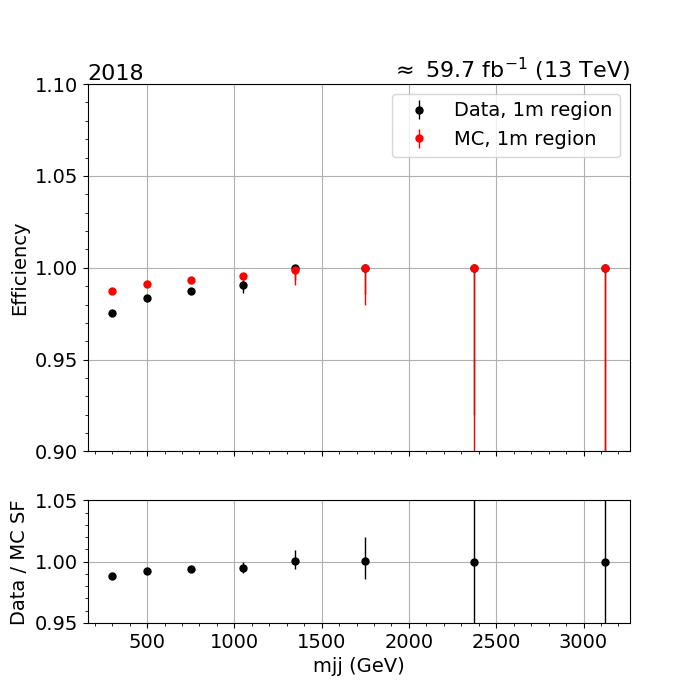
\includegraphics[width=0.49\textwidth]{fig/efficiency/trigger/met/mjj/data_mc_comparison_1m_2018_two_central_jets.png} \\
        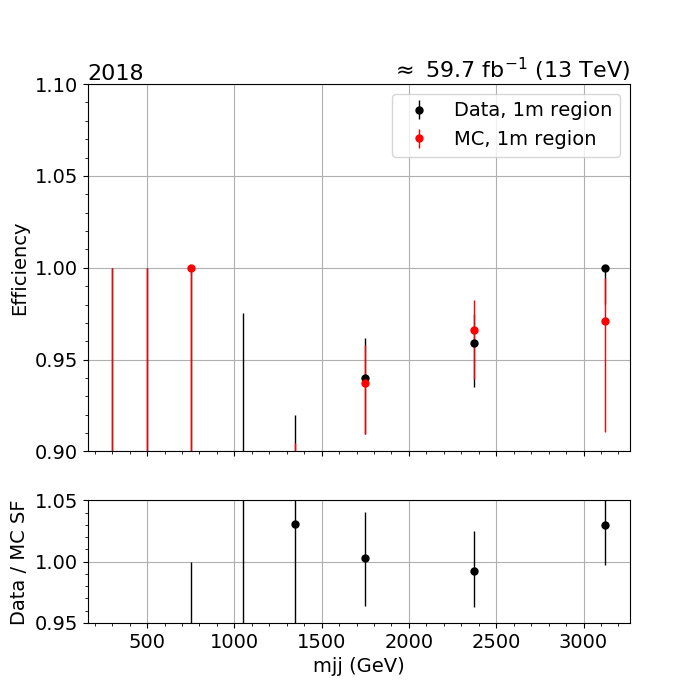
\includegraphics[width=0.49\textwidth]{fig/efficiency/trigger/met/mjj/data_mc_comparison_1m_2018_two_forward_jets.png}
    \end{center}
    \caption{MET trigger efficiency as a function of mjj in three categories: One forward jet and one central jet, two central jets and
            two forward jets. These results are obtained from 2018 data and MC samples with the selection of single muon events.}   
    \label{fig:eff_mjj_2018_1m}
\end{figure}

\begin{figure}[htp]
    \begin{center}
        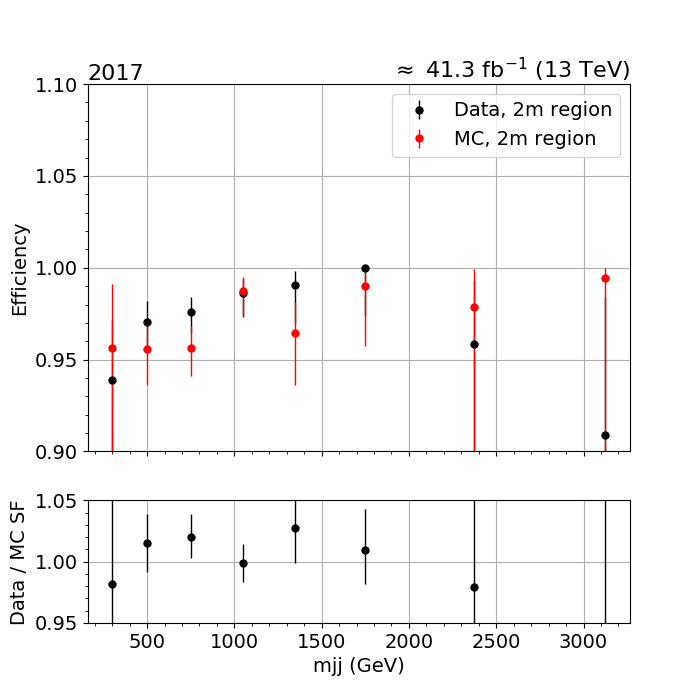
\includegraphics[width=0.49\textwidth]{fig/efficiency/trigger/met/mjj/data_mc_comparison_2m_2017_one_jet_forward_one_jet_central.png}
        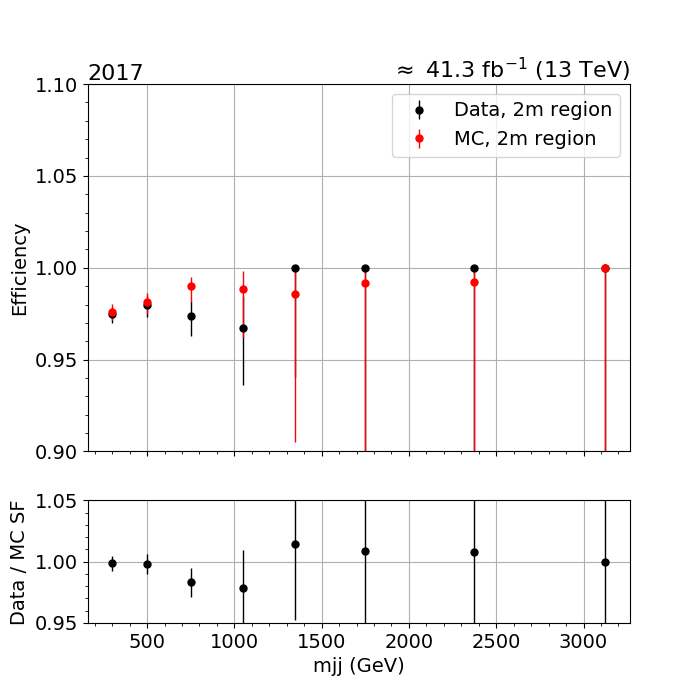
\includegraphics[width=0.49\textwidth]{fig/efficiency/trigger/met/mjj/data_mc_comparison_2m_2017_two_central_jets.png} \\
        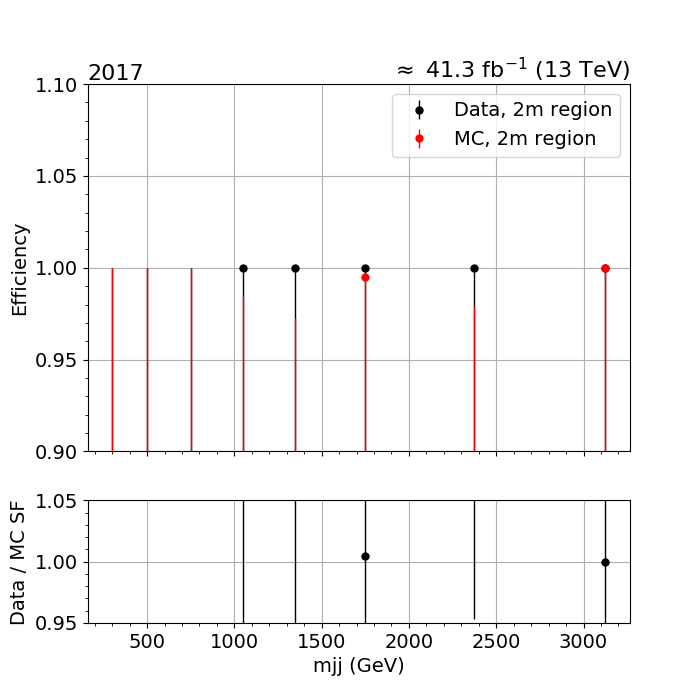
\includegraphics[width=0.49\textwidth]{fig/efficiency/trigger/met/mjj/data_mc_comparison_2m_2017_two_forward_jets.png}
    \end{center}
    \caption{MET trigger efficiency as a function of mjj in three categories: One forward jet and one central jet, two central jets and
            two forward jets. These results are obtained from 2017 data and MC samples with the selection of double muon events.}
    \label{fig:eff_mjj_2017_2m}
\end{figure}

\begin{figure}[hbp]
    \begin{center}
        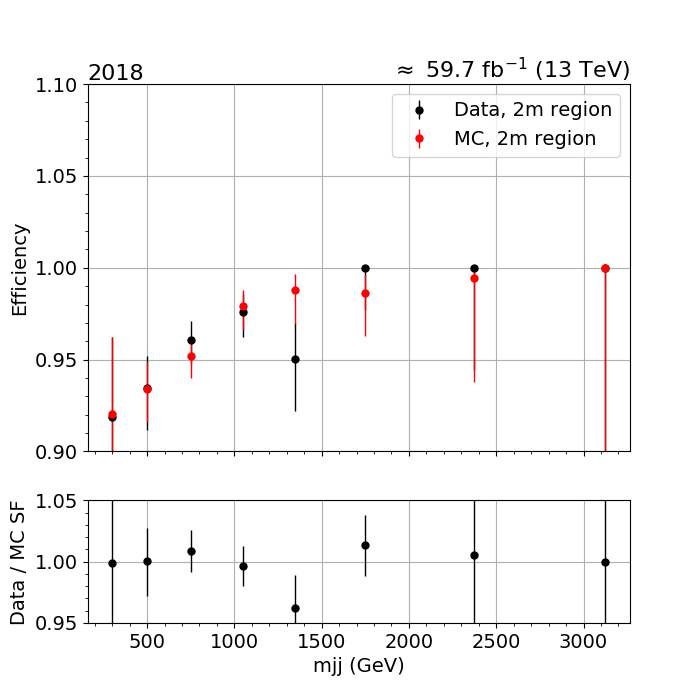
\includegraphics[width=0.49\textwidth]{fig/efficiency/trigger/met/mjj/data_mc_comparison_2m_2018_one_jet_forward_one_jet_central.png}
        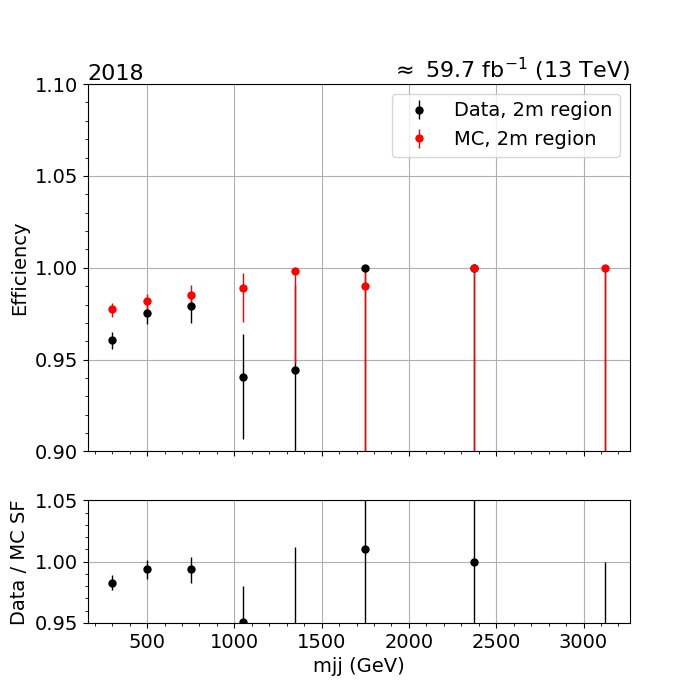
\includegraphics[width=0.49\textwidth]{fig/efficiency/trigger/met/mjj/data_mc_comparison_2m_2018_two_central_jets.png} \\
        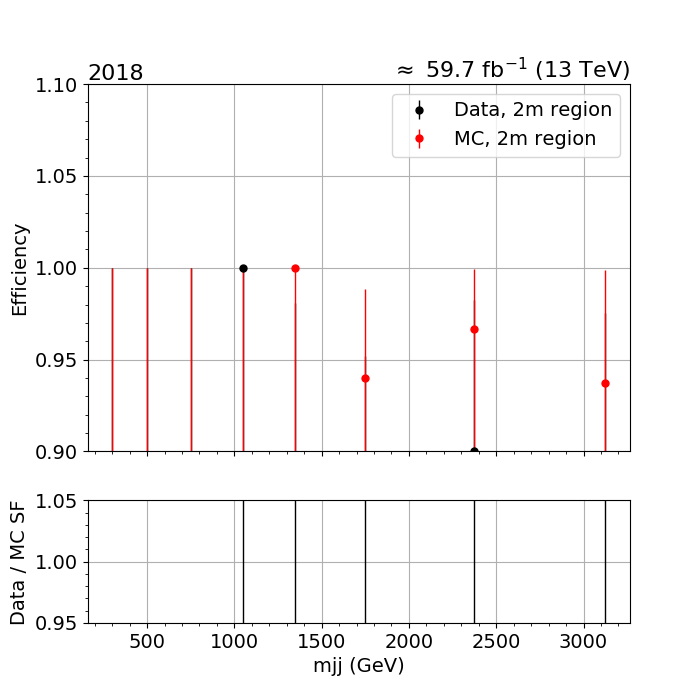
\includegraphics[width=0.49\textwidth]{fig/efficiency/trigger/met/mjj/data_mc_comparison_2m_2018_two_forward_jets.png}
    \end{center}
    \caption{MET trigger efficiency as a function of mjj in three categories: One forward jet and one central jet, two central jets and
            two forward jets. These results are obtained from 2018 data and MC samples with the selection of double muon events.}  
    \label{fig:eff_mjj_2018_2m}
\end{figure}

\begin{figure}[htp]
    \begin{center}
        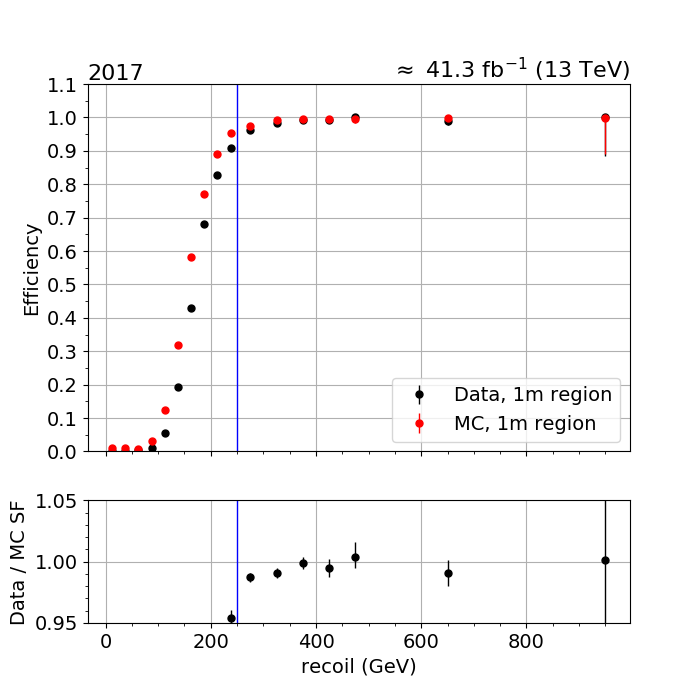
\includegraphics[width=0.49\textwidth]{fig/efficiency/trigger/met/recoil/data_mc_comparison_1m_2017_one_jet_forward_one_jet_central.png}
        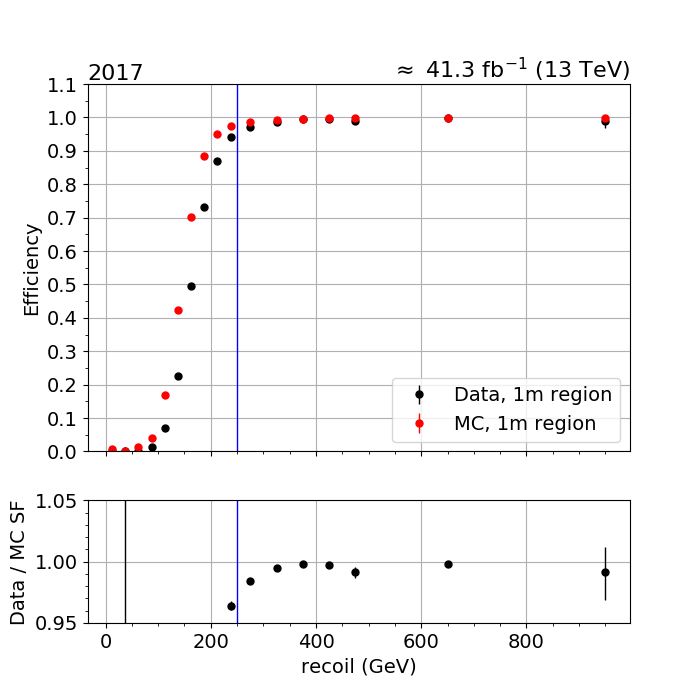
\includegraphics[width=0.49\textwidth]{fig/efficiency/trigger/met/recoil/data_mc_comparison_1m_2017_two_central_jets.png} \\
        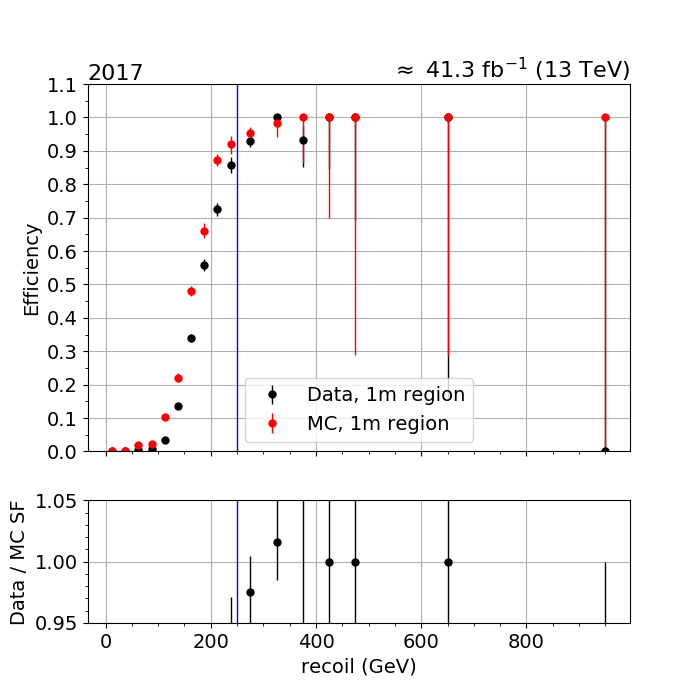
\includegraphics[width=0.49\textwidth]{fig/efficiency/trigger/met/recoil/data_mc_comparison_1m_2017_two_forward_jets.png}
    \end{center}
    \caption{MET trigger efficiency as a function of recoil in three categories: One forward jet and one central jet, two central jets and
            two forward jets. These results are obtained from 2017 data and MC samples with the selection of single muon events.} 
    \label{fig:eff_recoil_2017_1m}
\end{figure}

\begin{figure}[hbp]
    \begin{center}
        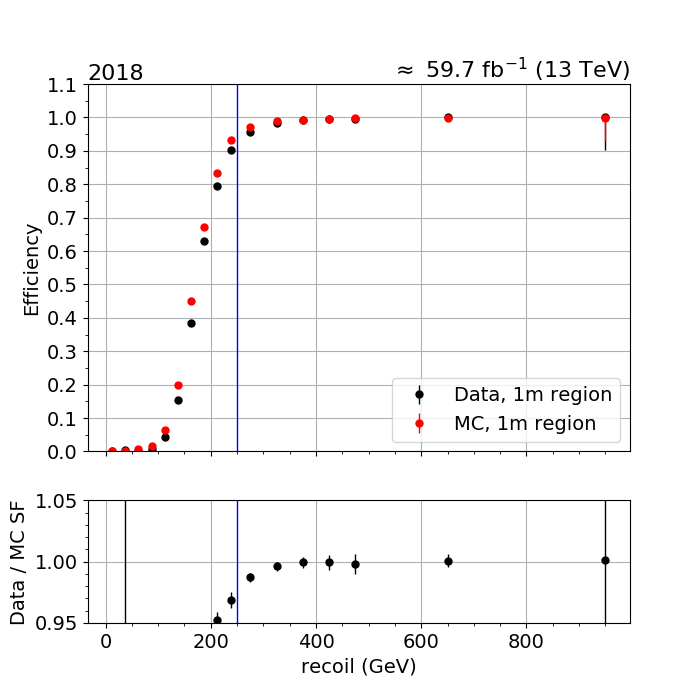
\includegraphics[width=0.49\textwidth]{fig/efficiency/trigger/met/recoil/data_mc_comparison_1m_2018_one_jet_forward_one_jet_central.png}
        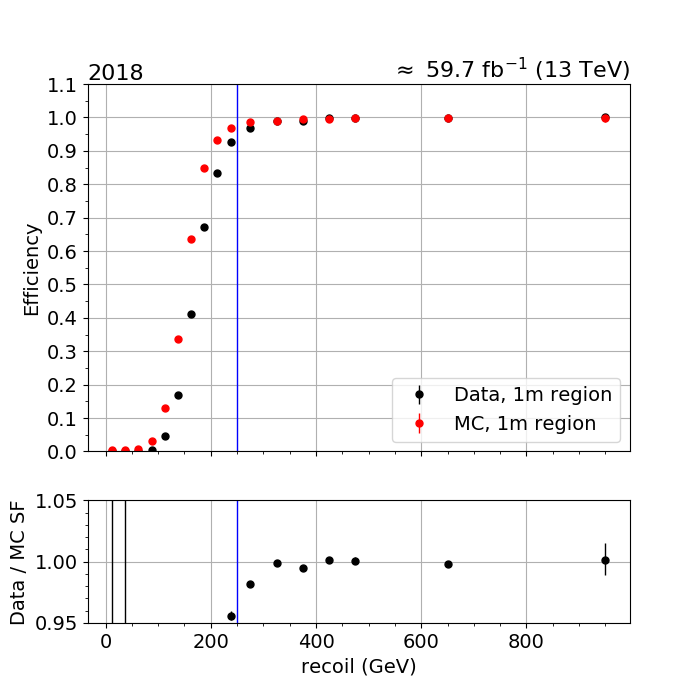
\includegraphics[width=0.49\textwidth]{fig/efficiency/trigger/met/recoil/data_mc_comparison_1m_2018_two_central_jets.png} \\
        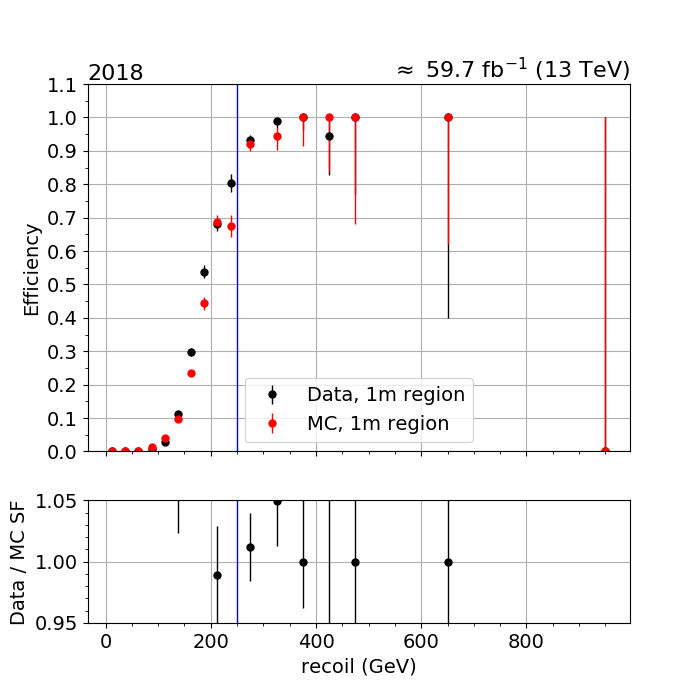
\includegraphics[width=0.49\textwidth]{fig/efficiency/trigger/met/recoil/data_mc_comparison_1m_2018_two_forward_jets.png}
    \end{center}
    \caption{MET trigger efficiency as a function of recoil in three categories: One forward jet and one central jet, two central jets and
            two forward jets. These results are obtained from 2018 data and MC samples with the selection of single muon events.}
    \label{fig:eff_recoil_2018_1m}
\end{figure}

\begin{figure}[htp]
    \begin{center}
        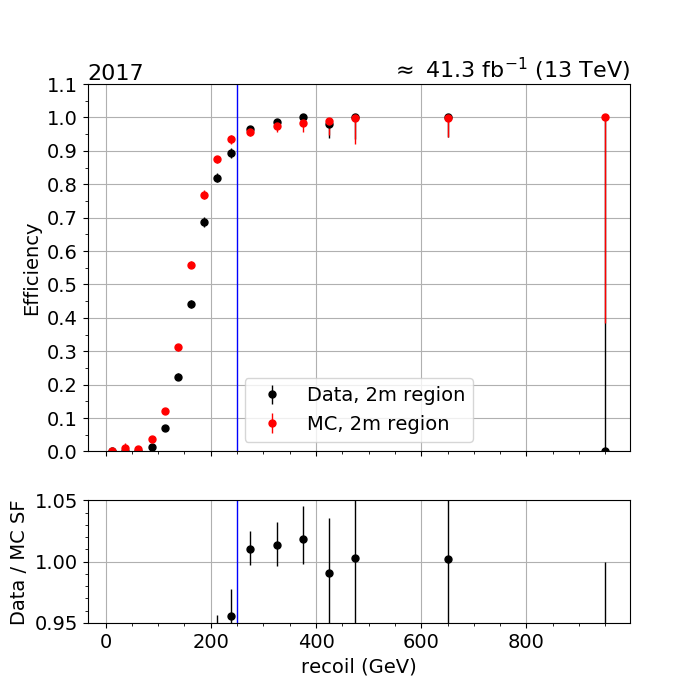
\includegraphics[width=0.49\textwidth]{fig/efficiency/trigger/met/recoil/data_mc_comparison_2m_2017_one_jet_forward_one_jet_central.png}
        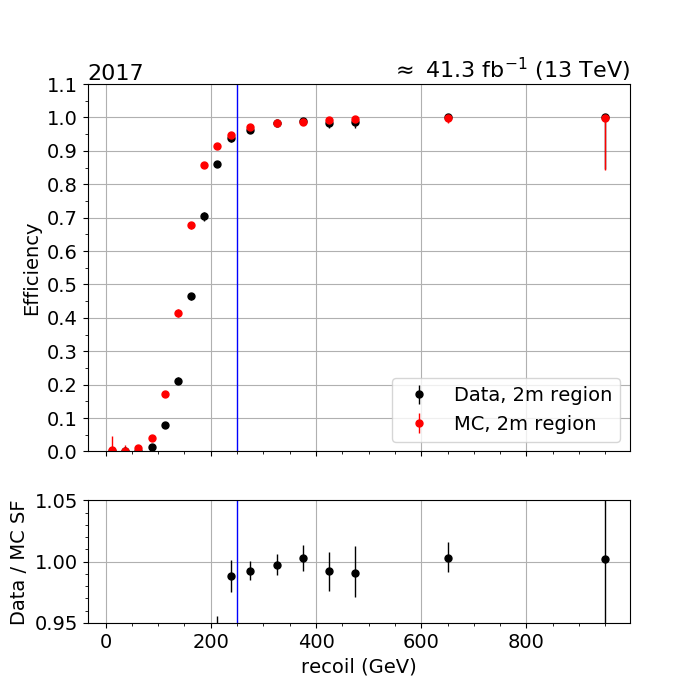
\includegraphics[width=0.49\textwidth]{fig/efficiency/trigger/met/recoil/data_mc_comparison_2m_2017_two_central_jets.png} \\
        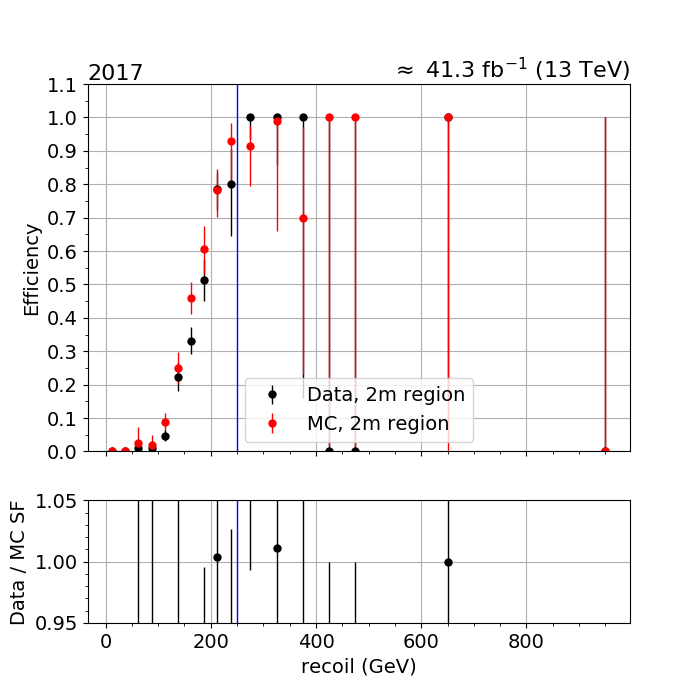
\includegraphics[width=0.49\textwidth]{fig/efficiency/trigger/met/recoil/data_mc_comparison_2m_2017_two_forward_jets.png}
    \end{center}
    \caption{MET trigger efficiency as a function of recoil in three categories: One forward jet and one central jet, two central jets and
            two forward jets. These results are obtained from 2017 data and MC samples with the selection of double muon events.}   
    \label{fig:eff_recoil_2017_2m}
\end{figure}

\begin{figure}[hbp]
    \begin{center}
        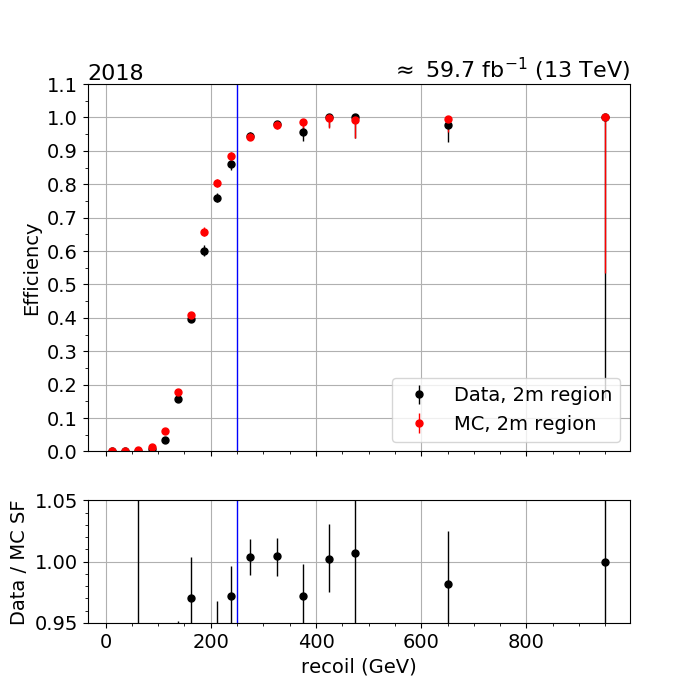
\includegraphics[width=0.49\textwidth]{fig/efficiency/trigger/met/recoil/data_mc_comparison_2m_2018_one_jet_forward_one_jet_central.png}
        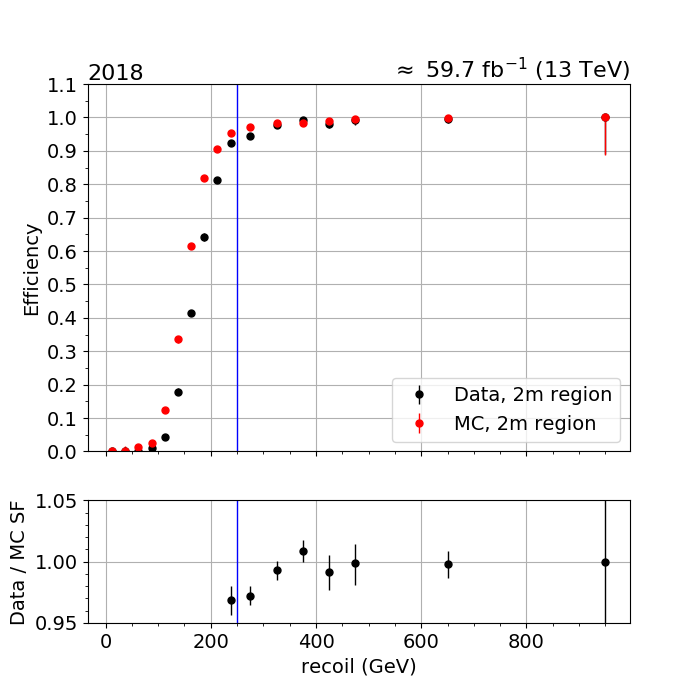
\includegraphics[width=0.49\textwidth]{fig/efficiency/trigger/met/recoil/data_mc_comparison_2m_2018_two_central_jets.png} \\
        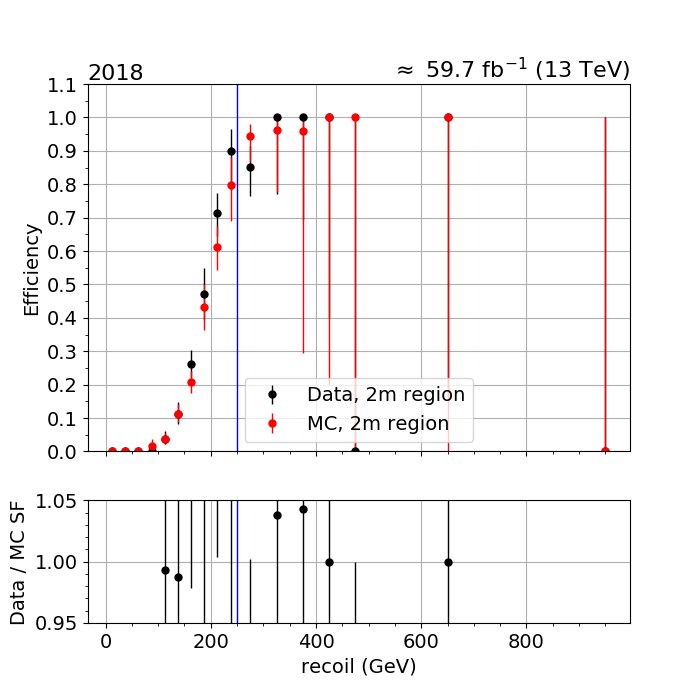
\includegraphics[width=0.49\textwidth]{fig/efficiency/trigger/met/recoil/data_mc_comparison_2m_2018_two_forward_jets.png}
    \end{center}
    \caption{MET trigger efficiency as a function of recoil in three categories: One forward jet and one central jet, two central jets and
            two forward jets. These results are obtained from 2018 data and MC samples with the selection of double muon events.}  
    \label{fig:eff_recoil_2018_2m}
\end{figure}